\documentclass[10pt]{article}
\usepackage[margin=1in]{geometry} 
\usepackage{enumerate, xfrac, color, graphicx}
\usepackage{amsmath,amsthm,amssymb,amsfonts,mathabx}
\usepackage{booktabs}
\usepackage{caption}
\usepackage{algorithm}
\usepackage{algpseudocode}
\usepackage{pifont}
\usepackage{listings, courier}
\graphicspath{{/Users/mfzhao/Dropbox/}}
\newcommand{\N}{\mathbb{N}}
\newcommand{\Z}{\mathbb{Z}}
\lstset{breaklines=true, basicstyle=\small\ttfamily, language=R, backgroundcolor=\color{highlight}, stepnumber=5}

\definecolor{highlight}{RGB}{248,248,248}

\begin{document}
	\title{6.867 Problem Set 2}
	\maketitle


\subsubsection*{Logistic Regression}
Here we want to predict the class of a discrete (or categorical) variable $Y$ given some some features $X$. While we can formulate this classification problem in the context of the linear regression framework we're already familiar with (these are known as linear probability models), these classical linear models are generally unbounded which may not be the best choice for modeling probabilities. Rather, we consider a slightly modified version of linear regression where we take the standard linear prediction $w_o + \sum_i w_i x_i$ and transform it such that it is bounded on $[0,1]$. In our case, our choice of a transformation function is the sigmoid function:
\begin{equation*}
	\sigma(z) = \frac{1}{1+e^{z}}
\end{equation*}

This transformed model is known as logistic or logit regression. Using this formulation, our the negative log-likelihood becomes:
\begin{equation*}
	\textnormal{NLL}=\sum_i \log \left(1+e^{-y^{(i)}(w_0 + x^{(i)}\cdot w)} \right)
\end{equation*}
We think that overfitting might be problem in logistic regression especially in the case of linearly separable data which will drive our weights $w$ to very large values to minimize the the logistic loss. Hence, we add a ridge penalty to the weights:
\begin{equation*}
	\min_w \sum_i \log \left(1+e^{-y^{(i)}(w_0 + x^{(i)}\cdot w)} \right) + \lambda w^T w
\end{equation*}
Using this, we trained Logistic Regressions for each of our 4 datasets using gradient descent. The optimal weights are reported below:

\begin{table}[ht]
\centering
\captionof{table}{Optimal Weights Trained on Various Datasets}
\begin{tabular}{lrrrr}
\toprule
{}    &      stdev1 &    stdev2 &    stdev4 & nonsep\\
\midrule
$w_0$ &  -63.930971 & -0.009267 & -0.046649 & 0.000597\\
$w_1$ &  266.198033 &  0.236279 &  0.763589 & -0.024737\\
$w_2$ &  160.999118 &  0.203428 &  1.114811 & -0.023726\\
\bottomrule
\end{tabular}
\end{table}

Logistic regression produces a predicted probability of a class rather than an actual classification. This means that we need to decide a decision boundary to minimizes our classifcation error. Considering we have symmetric loss, we intuitively might want our decision boundary to be 0.5 which produces the following error rates:

\begin{table}[ht]
\centering
\captionof{table}{Performance of Logistic Regression with Decision boundary of 0.5}
\begin{tabular}{lrrrr}
\toprule
{} & stdev1 & stdev2 & stdev4 & nonsep\\
\midrule
  Training Error   & 0.00\%  & 9.25\% &  26.00\% & 48.50\% \\
  Validation Error & 0.00\%  & 8.00\% &  24.75\% & 50.75\% \\
\bottomrule
\end{tabular}
\end{table}


These results make a lot of sense as we should expect the classification error to be 0 for the perfectly linearly separable case and get progressively worse as as the two classes overlap. In fact, in the nonseparable case, our classifier is no better (or even slightly worse) than random guessing! We can see this as we plot our decision boundary in X-space below:

\begin{figure}[ht]
	\centering
	\begin{minipage}[b]{.24\linewidth}
		\centering
		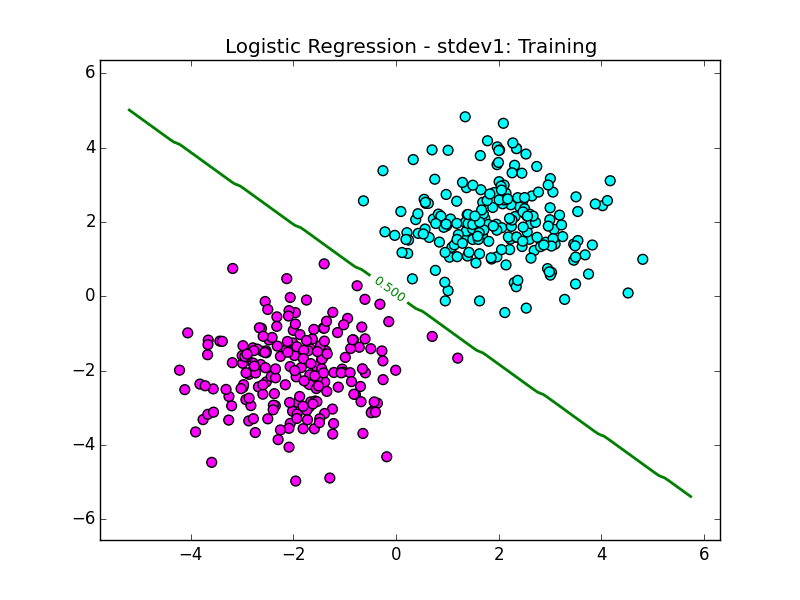
\includegraphics[width=.5\linewidth, height=.5in]{LR_stdev1_train.png}
		\caption*{stdev1 (Training)}
	\end{minipage}
	\begin{minipage}[b]{.24\linewidth}
		\centering
		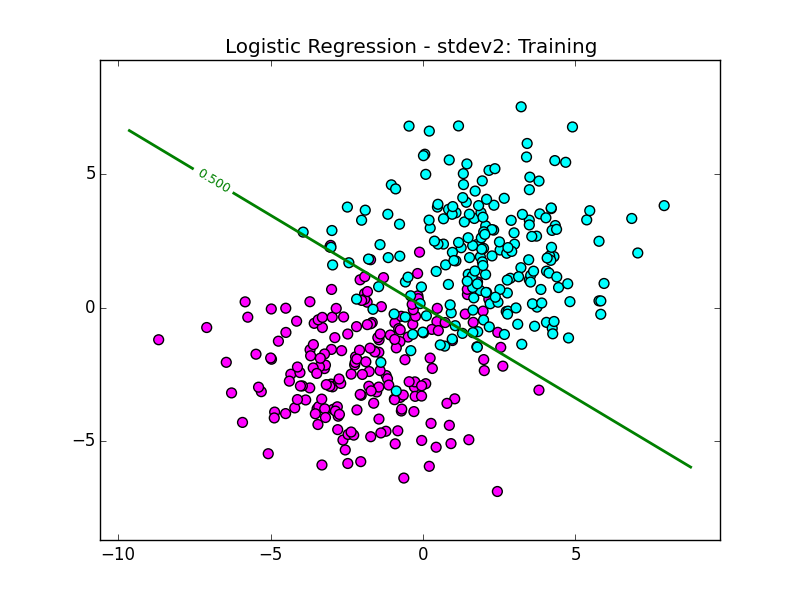
\includegraphics[width=.5\linewidth, height=.5in]{LR_stdev2_train.png}
		\caption*{stdev2 (Training)}
	\end{minipage}
	\begin{minipage}[b]{.24\linewidth}
		\centering
		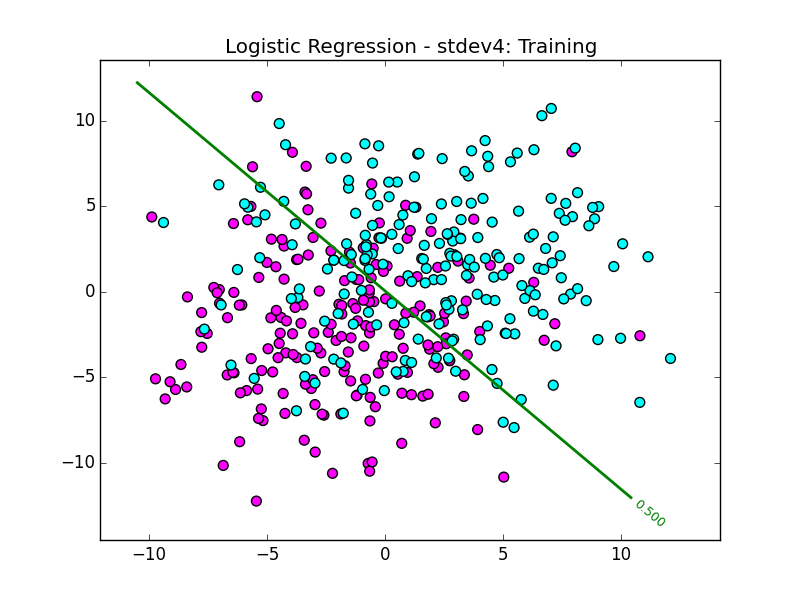
\includegraphics[width=.5\linewidth, height=.5in]{LR_stdev4_train.png}
		\caption*{stdev4 (Training)}
	\end{minipage}
	\begin{minipage}[b]{.24\linewidth}
		\centering
		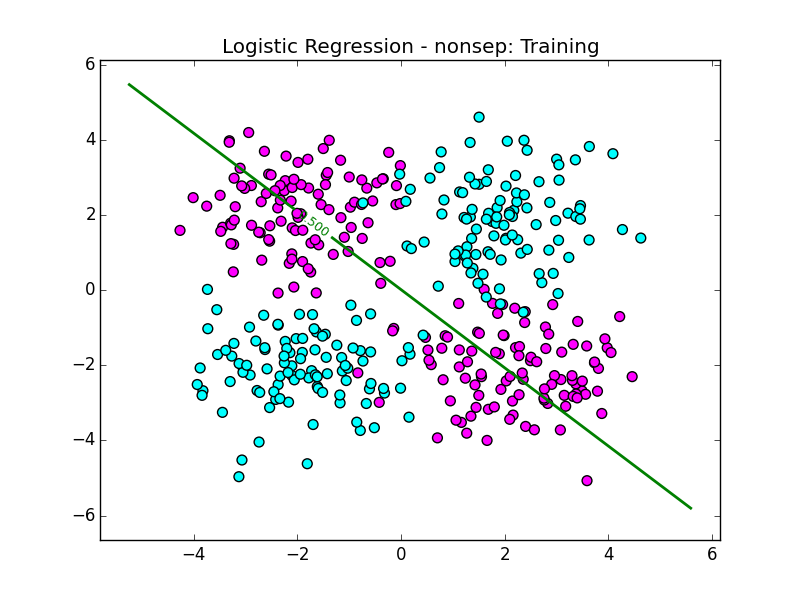
\includegraphics[width=.5\linewidth, height=.5in]{LR_nonsep_train.png}
		\caption*{nonsep (Training)}
	\end{minipage}
		\begin{minipage}[b]{.24\linewidth}
		\centering
		\includegraphics[width=.5\linewidth, height=.5in]{LR_stdev1_validation.png}
		\caption*{stdev1 (Validation)}
	\end{minipage}
	\begin{minipage}[b]{.24\linewidth}
		\centering
		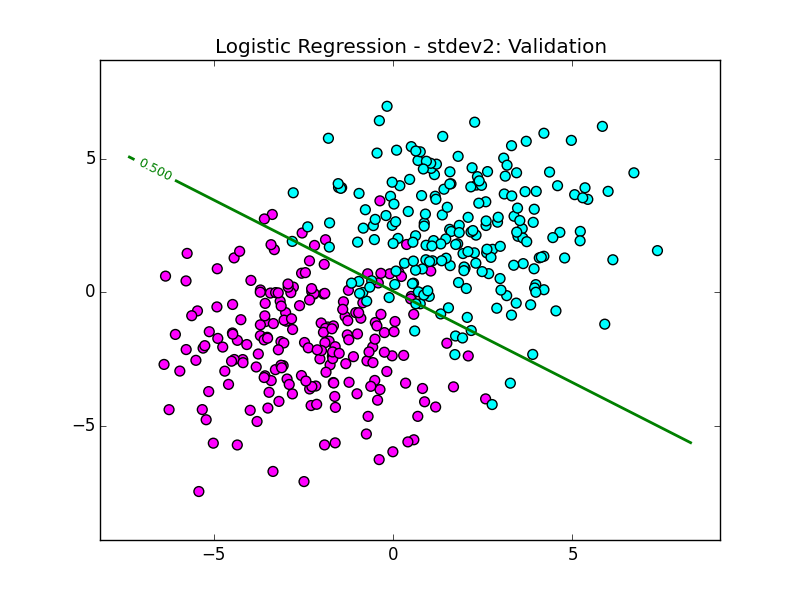
\includegraphics[width=.5\linewidth, height=.5in]{LR_stdev2_validation.png}
		\caption*{stdev2 (Validation)}
	\end{minipage}
	\begin{minipage}[b]{.24\linewidth}
		\centering
		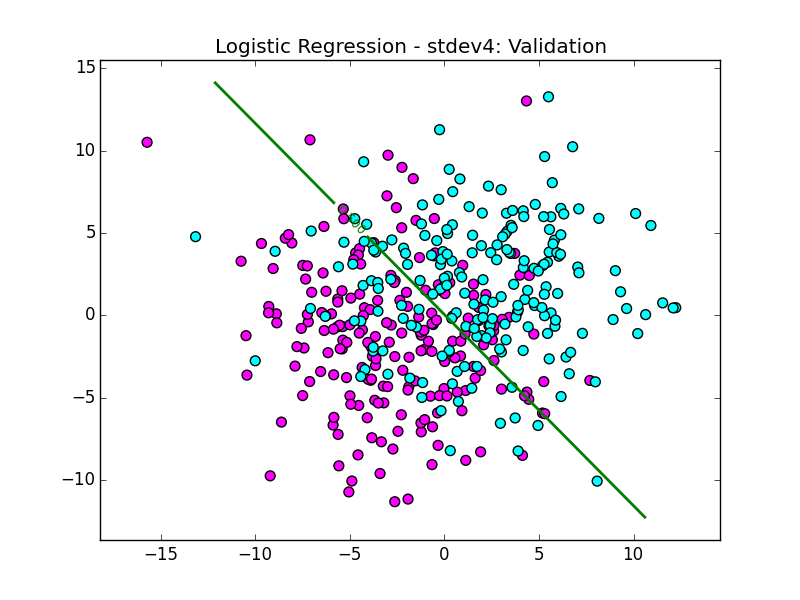
\includegraphics[width=.5\linewidth, height=.5in]{LR_stdev4_validation.png}
		\caption*{stdev4 (Validation)}
	\end{minipage}
	\begin{minipage}[b]{.24\linewidth}
		\centering
		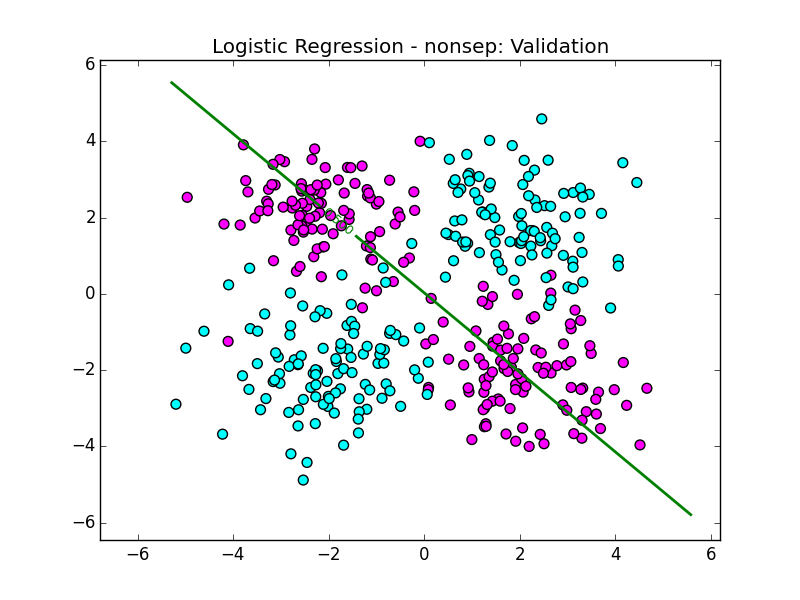
\includegraphics[width=.5\linewidth, height=.5in]{LR_nonsep_validation.png}
		\caption*{nonsep (Validation)}
	\end{minipage}
	\caption{The decision boundaries generated by Logistic Regression plotted against the stdev1, stdev2, stdev4, and nonsep (training and validation) datasets}
\end{figure}

We are also interested in examining classification error as we vary our choice of the decision boundary. This is depicted in in figure 2 below:

\begin{figure}[ht]
	\centering
	\begin{minipage}[b]{.24\linewidth}
		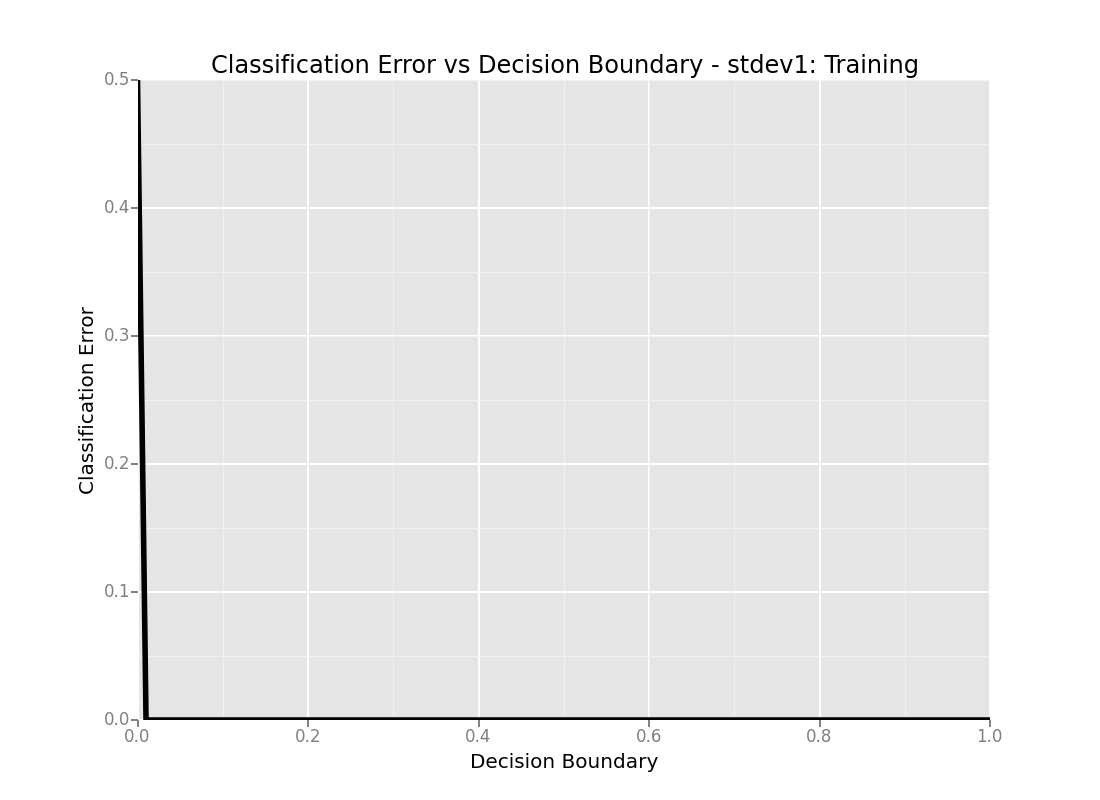
\includegraphics[width=1\linewidth, height=1in]{CEDB_stdev1_train.png}
		\caption*{stdev1 (Training)}
	\end{minipage}
	\begin{minipage}[b]{.24\linewidth}
		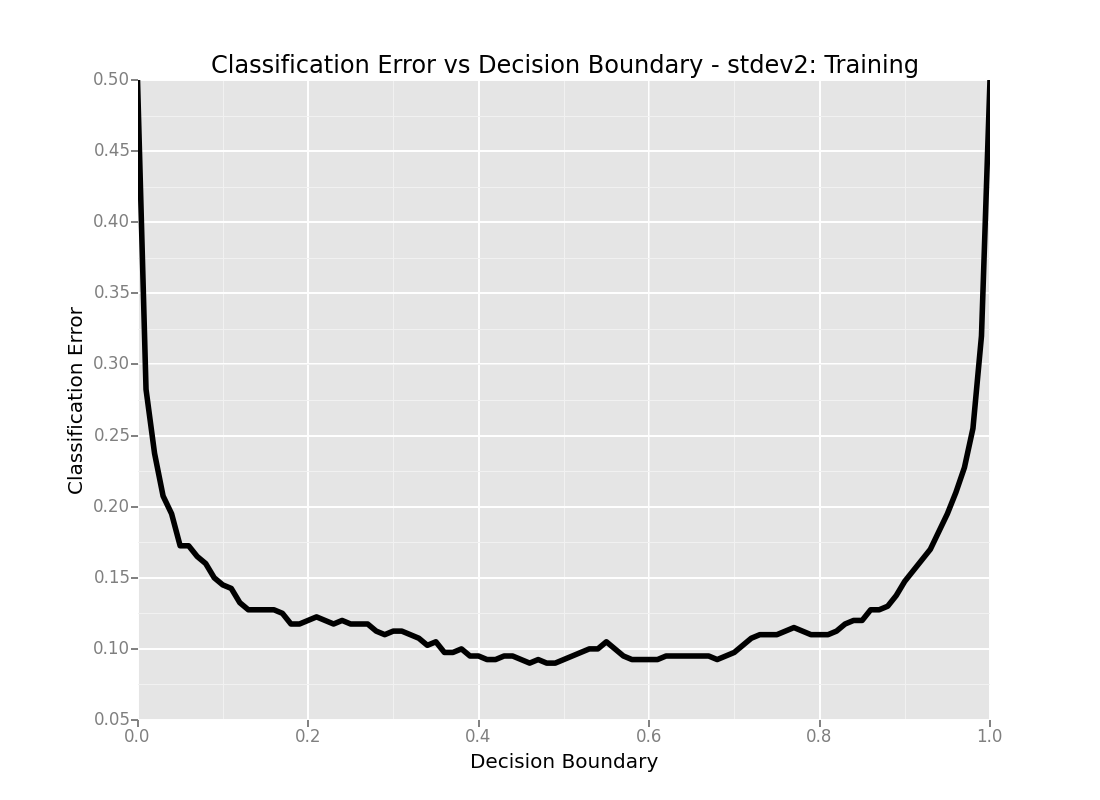
\includegraphics[width=1\linewidth, height=1in]{CEDB_stdev2_train.png}
		\caption*{stdev2 (Training)}
	\end{minipage}
	\begin{minipage}[b]{.24\linewidth}
		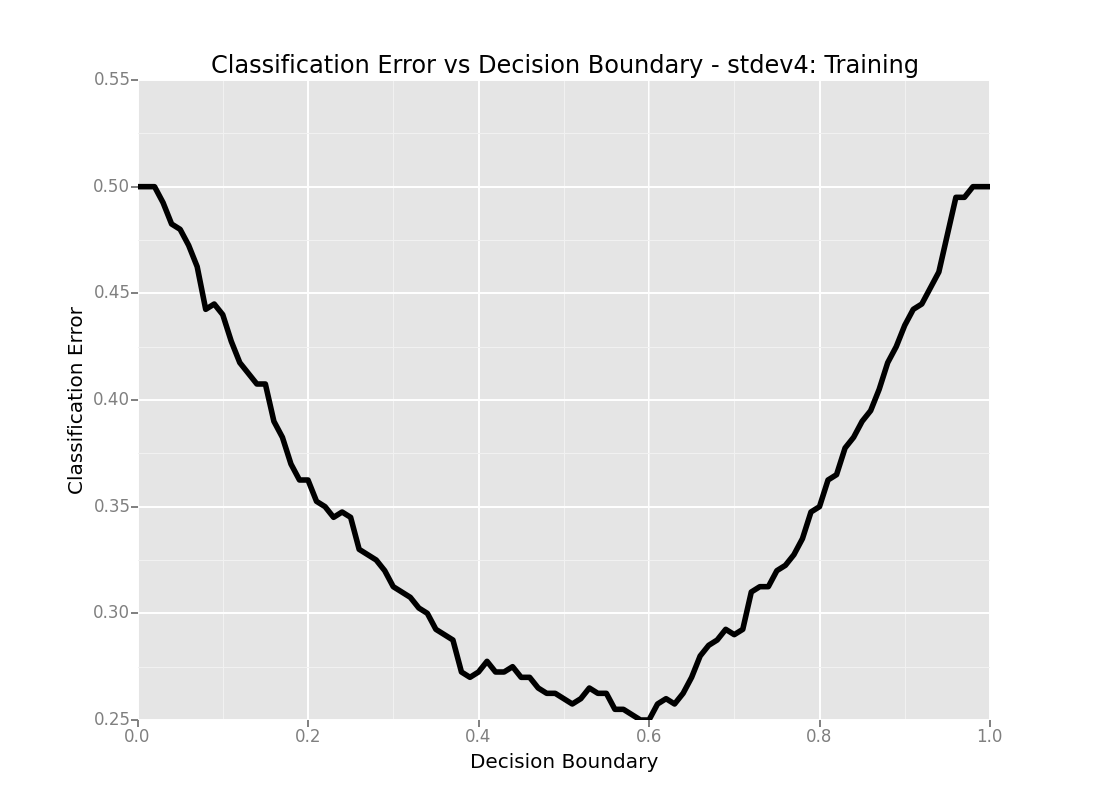
\includegraphics[width=1\linewidth, height=1in]{CEDB_stdev4_train.png}
		\caption*{stdev4 (Training)}
	\end{minipage}
	\begin{minipage}[b]{.24\linewidth}
		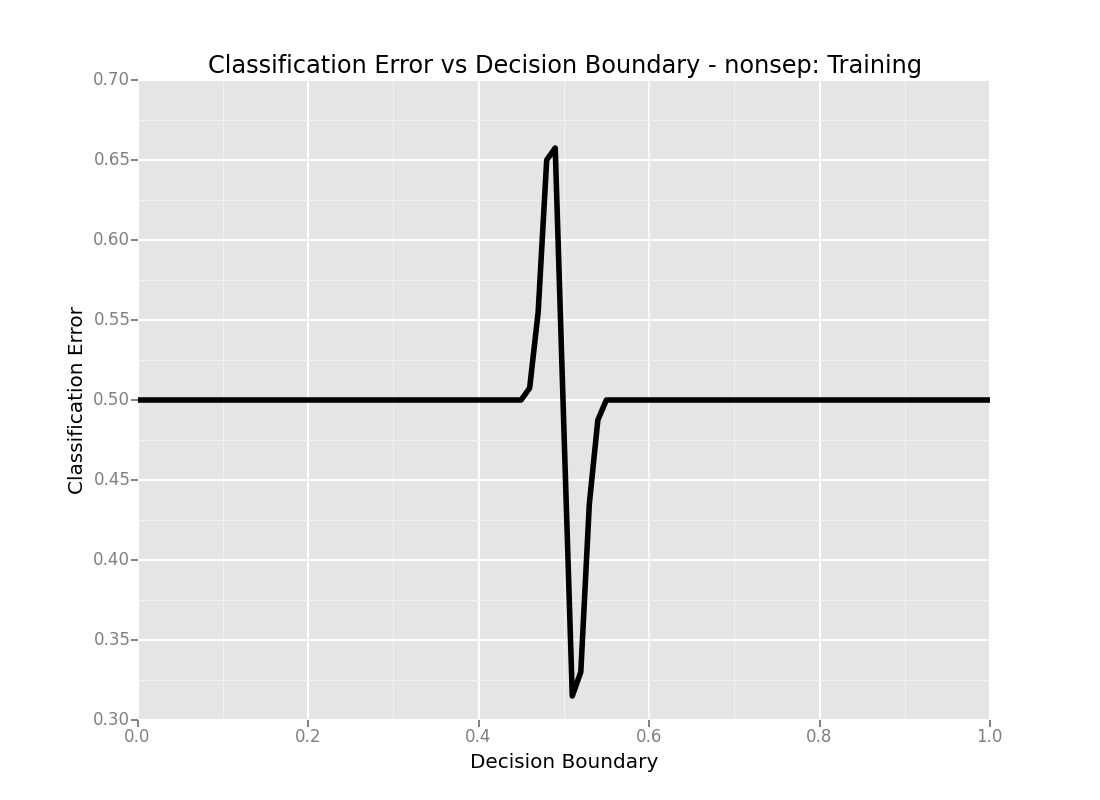
\includegraphics[width=1\linewidth, height=1in]{CEDB_nonsep_train.png}
		\caption*{nonsep (Training)}
	\end{minipage}
		\begin{minipage}[b]{.24\linewidth}
		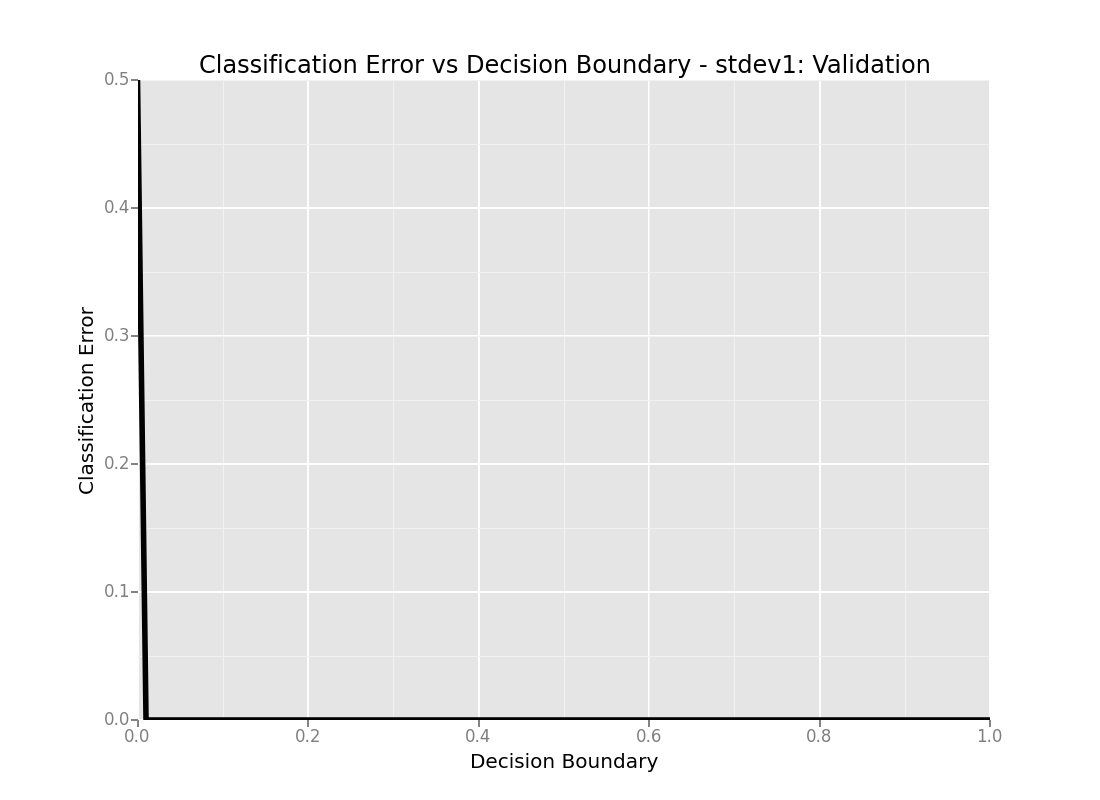
\includegraphics[width=1\linewidth, height=1in]{CEDB_stdev1_validation.png}
		\caption*{stdev1 (Validation)}
	\end{minipage}
	\begin{minipage}[b]{.24\linewidth}
		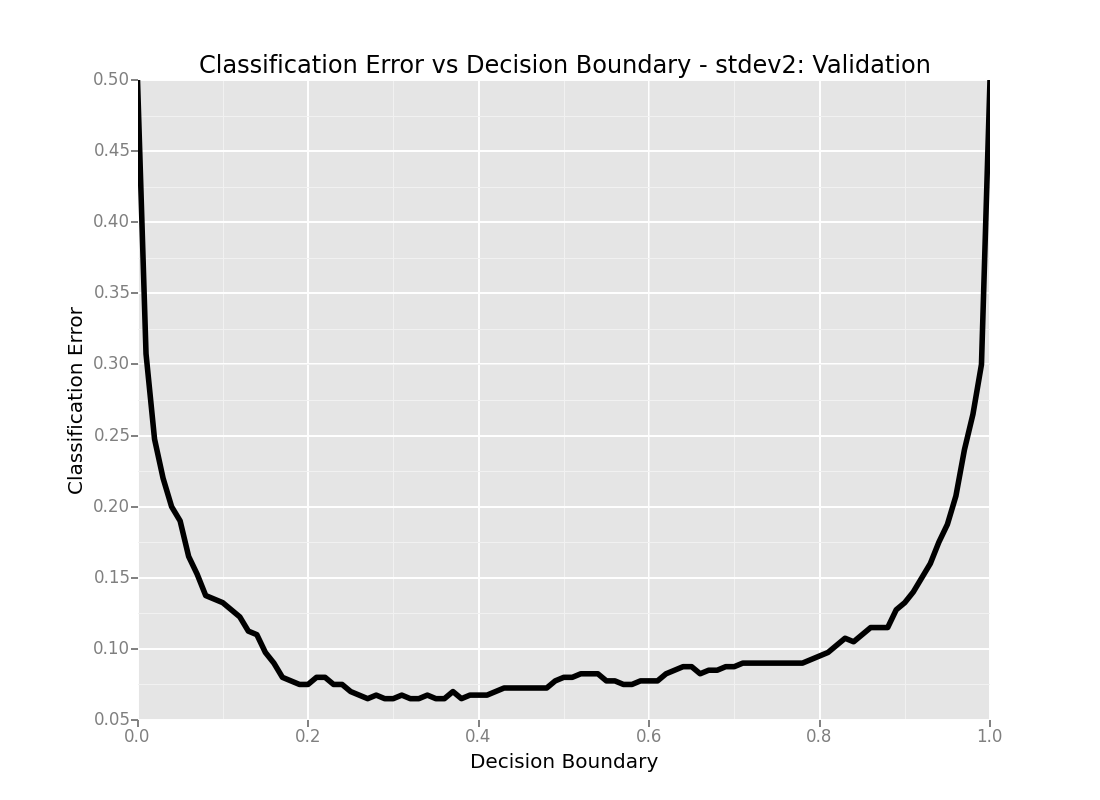
\includegraphics[width=1\linewidth, height=1in]{CEDB_stdev2_validation.png}
		\caption*{stdev2 (Validation)}
	\end{minipage}
	\begin{minipage}[b]{.24\linewidth}
		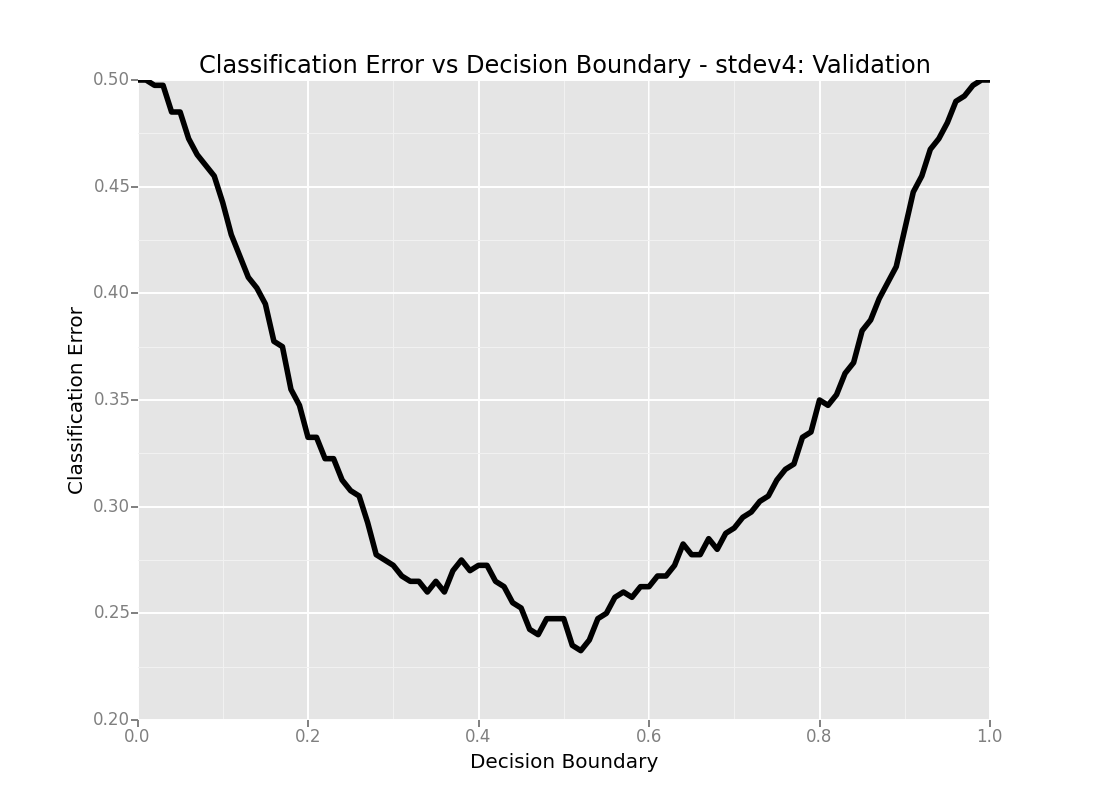
\includegraphics[width=1\linewidth, height=1in]{CEDB_stdev4_validation.png}
		\caption*{stdev4 (Validation)}
	\end{minipage}
	\begin{minipage}[b]{.24\linewidth}
		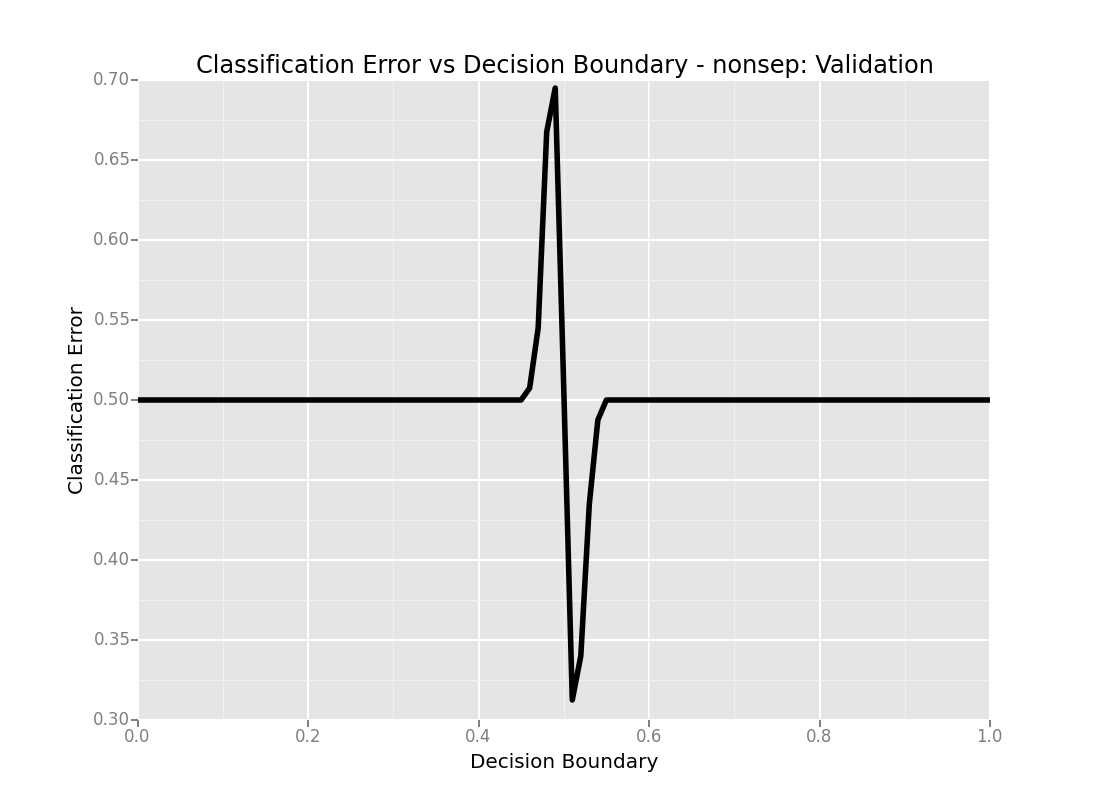
\includegraphics[width=1\linewidth, height=1in]{CEDB_nonsep_validation.png}
		\caption*{nonsep (Validation)}
	\end{minipage}
	\caption{The classification error of Logistic Regression as a function of our choice of a decision boundary for the stdev1, stdev2, stdev4, and nonsep (training and validation) datasets}
\end{figure}

In the linearly separable case (stdev1), we see that just about any value greater than 0 gives us perfect classification, which makes intuitive sense since the optimal weights will try to push everything to either 0 or 1 resulting in the graph we see: the error starts out at .5 and almost immediately drops to 0. However if the data is still generally but not perfectly linearly separable (stdev2 and stdev4), we get what we would expect--classification error starts high and decreases until around decision boundary of 0.5 and then starts to increase again. In the linearly non-seperable case (nonsep), the probabilities are all relatively close to 0.5. Hence we don't see any effect of changing the decision boundary until we get relatively close to 0.5 in this case, we see that we get a spike since we start to misclassify the green points while all the purple points are still incorrectly classified. The spike drops back to 0.5 at around decision boundary of 0.5 and decreases as we start to correctly classify all the purple points. As we continue to increase the decision boundary, we get to the case were we classify everything as purple leading us with a misclassification rate of 0.5. 

We also explore the effect of adding a ridge penalty to logistic regression. We plot the classification error and loss of our regression as a function of the penalty $\lambda$:

\begin{figure}[ht]
	\centering
	\begin{minipage}[b]{.24\linewidth}
		\centering
		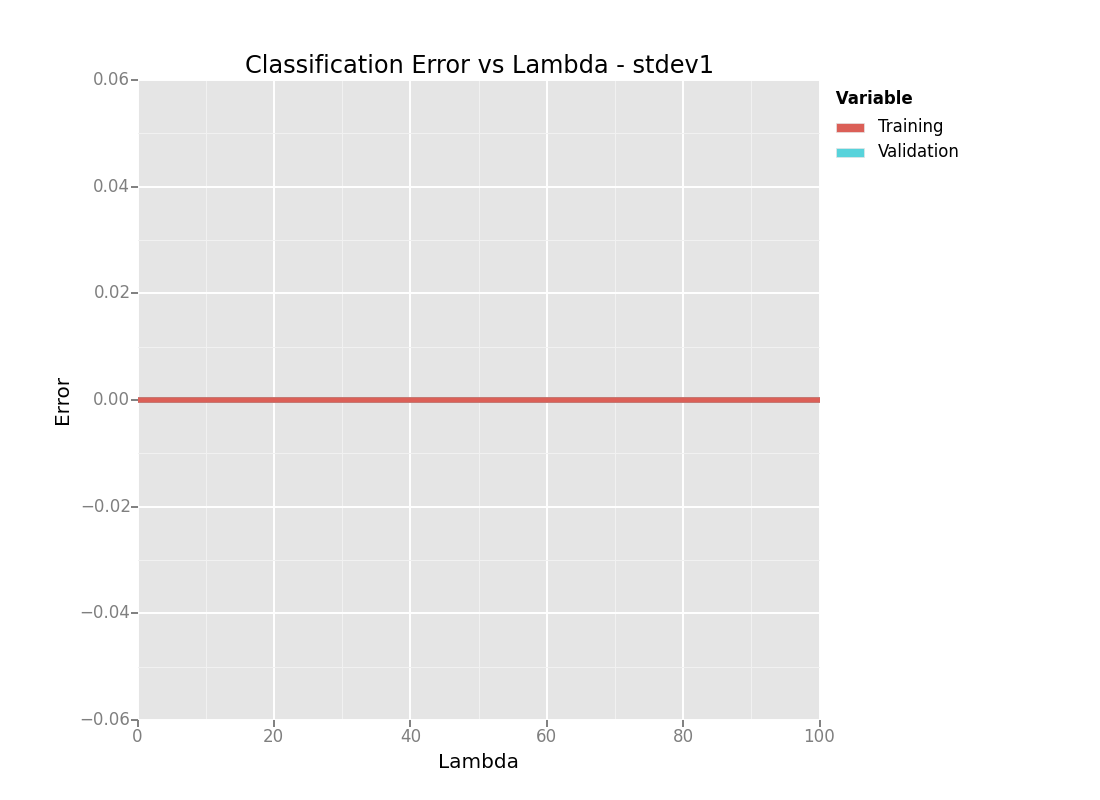
\includegraphics[width=.5\linewidth, height=.5in]{CErr_lambda_stdev1.png}
		\caption*{Error - stdev1}
	\end{minipage}
	\begin{minipage}[b]{.24\linewidth}
		\centering
		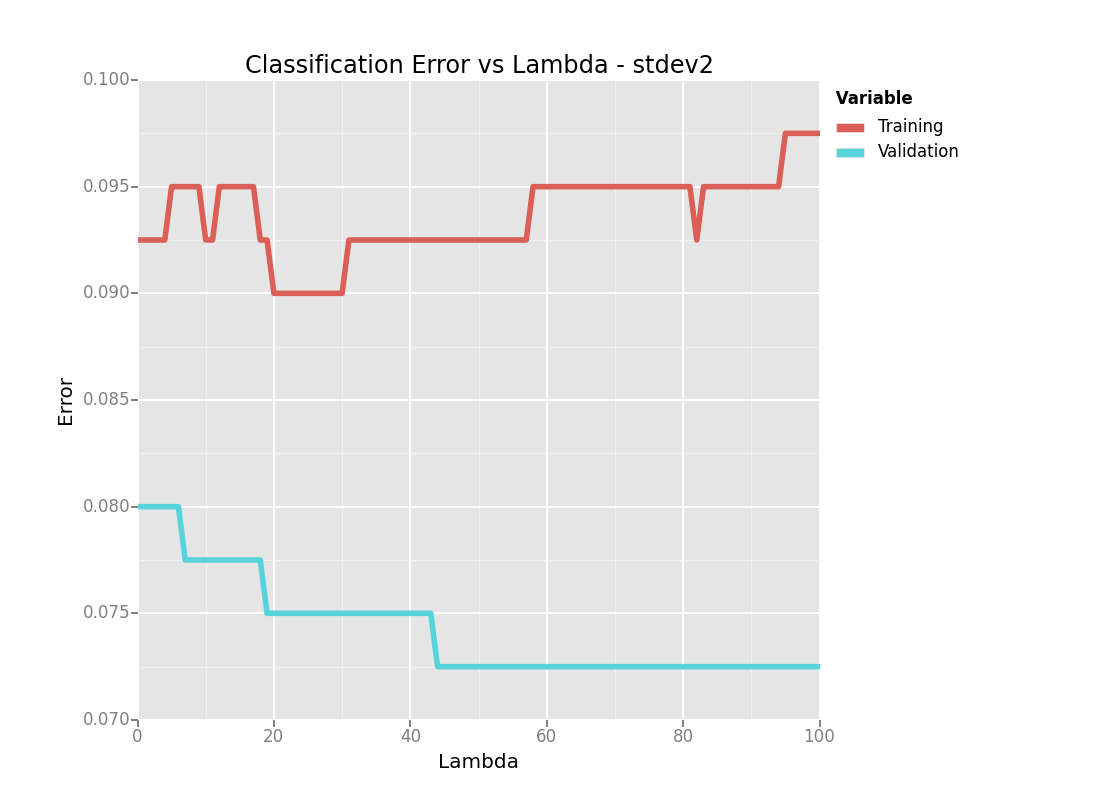
\includegraphics[width=.5\linewidth, height=.5in]{CErr_lambda_stdev2.png}
		\caption*{Error - stdev2}
	\end{minipage}
	\begin{minipage}[b]{.24\linewidth}
		\centering
		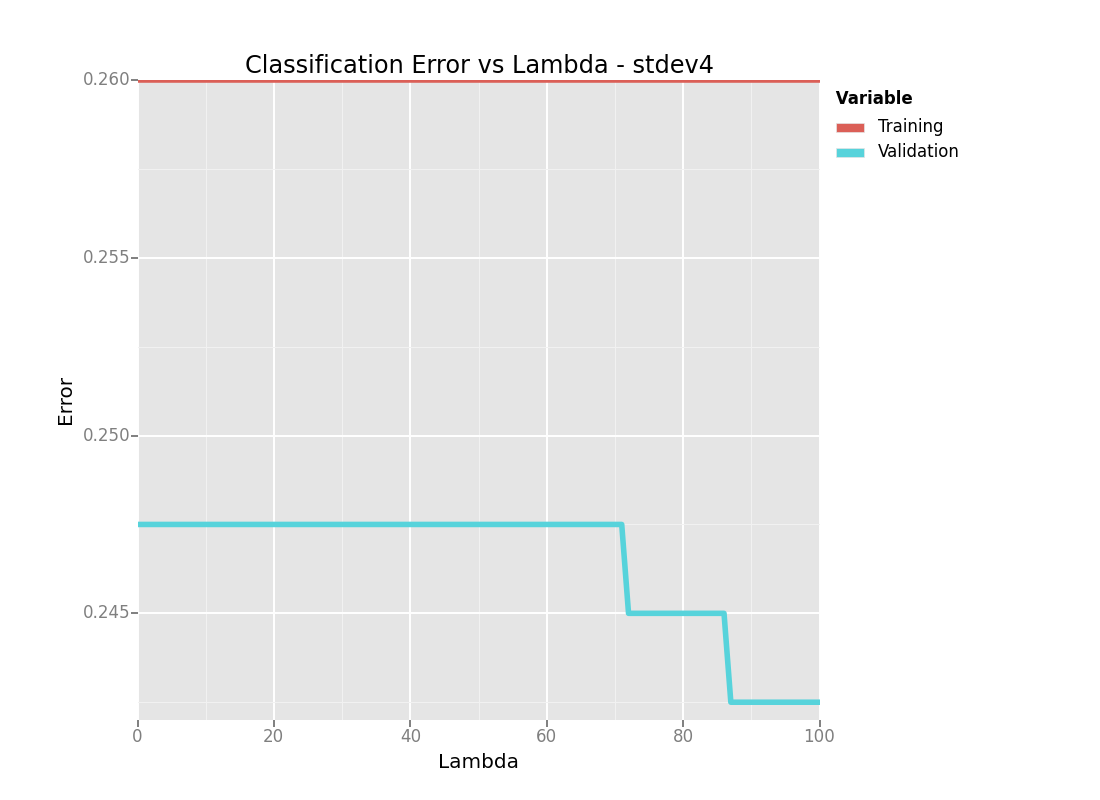
\includegraphics[width=.5\linewidth, height=.5in]{CErr_lambda_stdev4.png}
		\caption*{Error - stdev4}
	\end{minipage}
	\begin{minipage}[b]{.24\linewidth}
		\centering
		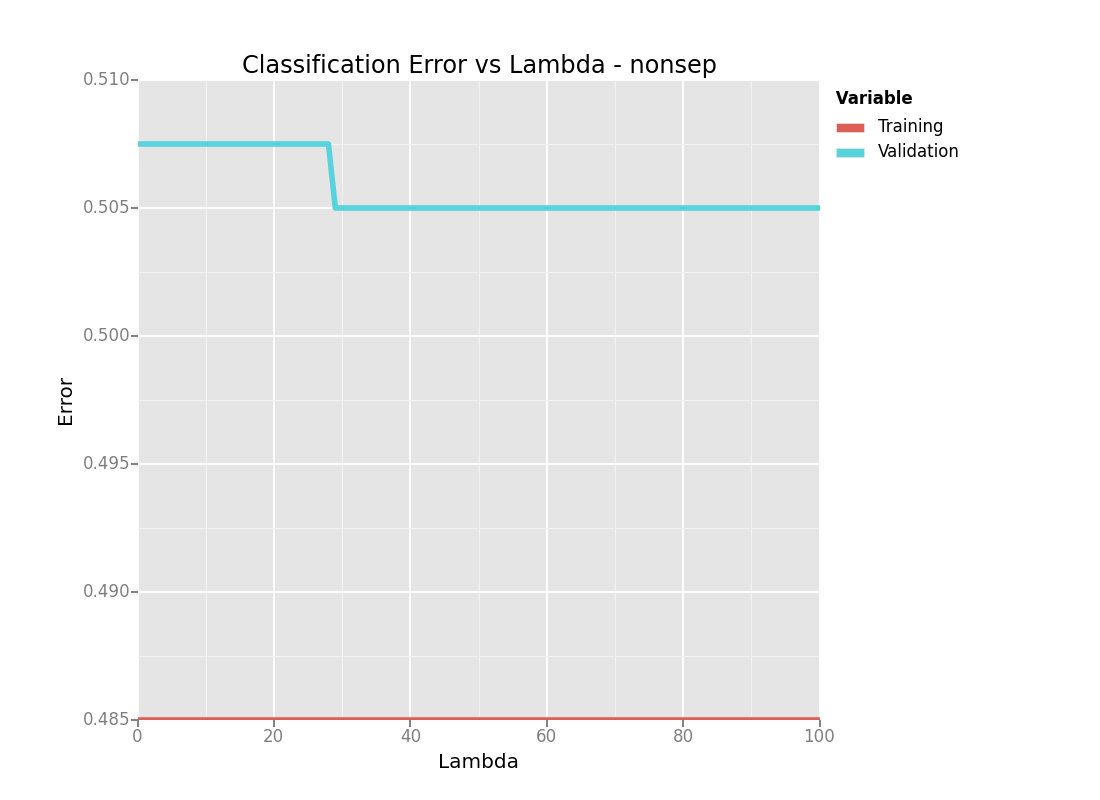
\includegraphics[width=.5\linewidth, height=.5in]{CErr_lambda_nonsep.png}
		\caption*{Error - nonsep}
	\end{minipage}
		\begin{minipage}[b]{.24\linewidth}
		\centering
		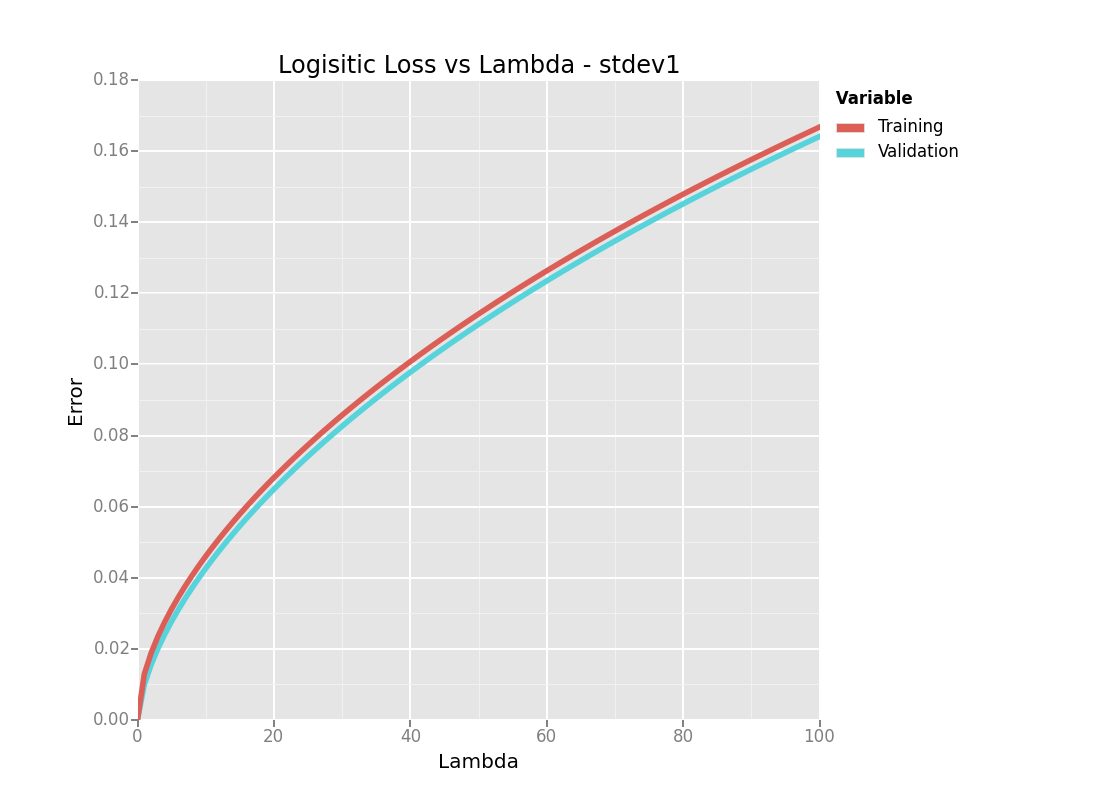
\includegraphics[width=.5\linewidth, height=.5in]{Loss_lambda_stdev1.png}
		\caption*{Logistic Loss - stdev1}
	\end{minipage}
	\begin{minipage}[b]{.24\linewidth}
		\centering
		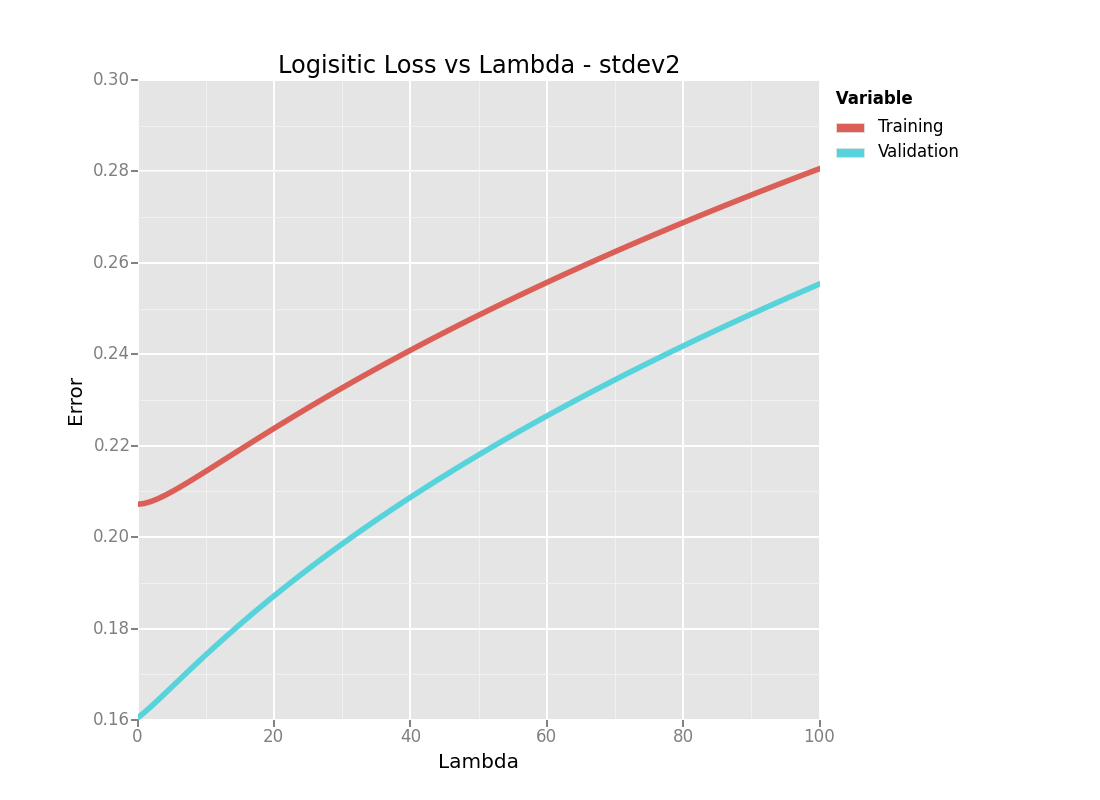
\includegraphics[width=.5\linewidth, height=.5in]{Loss_lambda_stdev2.png}
		\caption*{Logistic Loss - stdev2}
	\end{minipage}
	\begin{minipage}[b]{.24\linewidth}
		\centering
		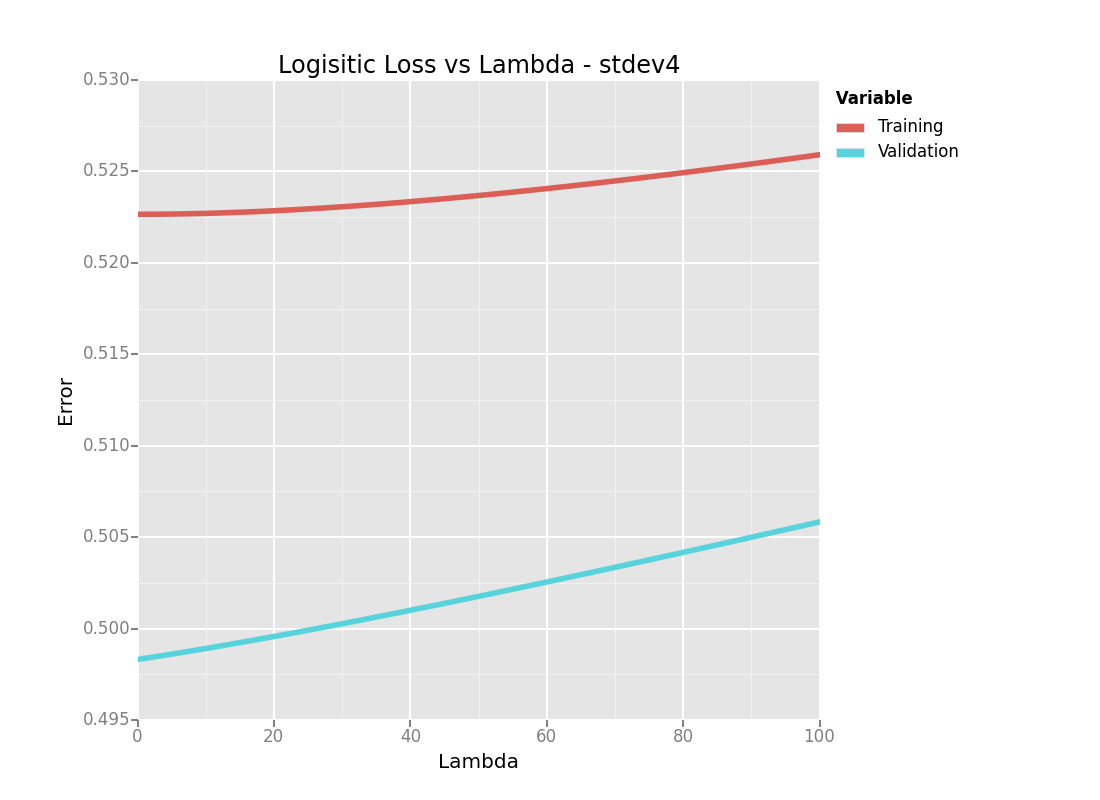
\includegraphics[width=.5\linewidth, height=.5in]{Loss_lambda_stdev4.png}
		\caption*{Logistic Loss - stdev4}
	\end{minipage}
	\begin{minipage}[b]{.24\linewidth}
		\centering
		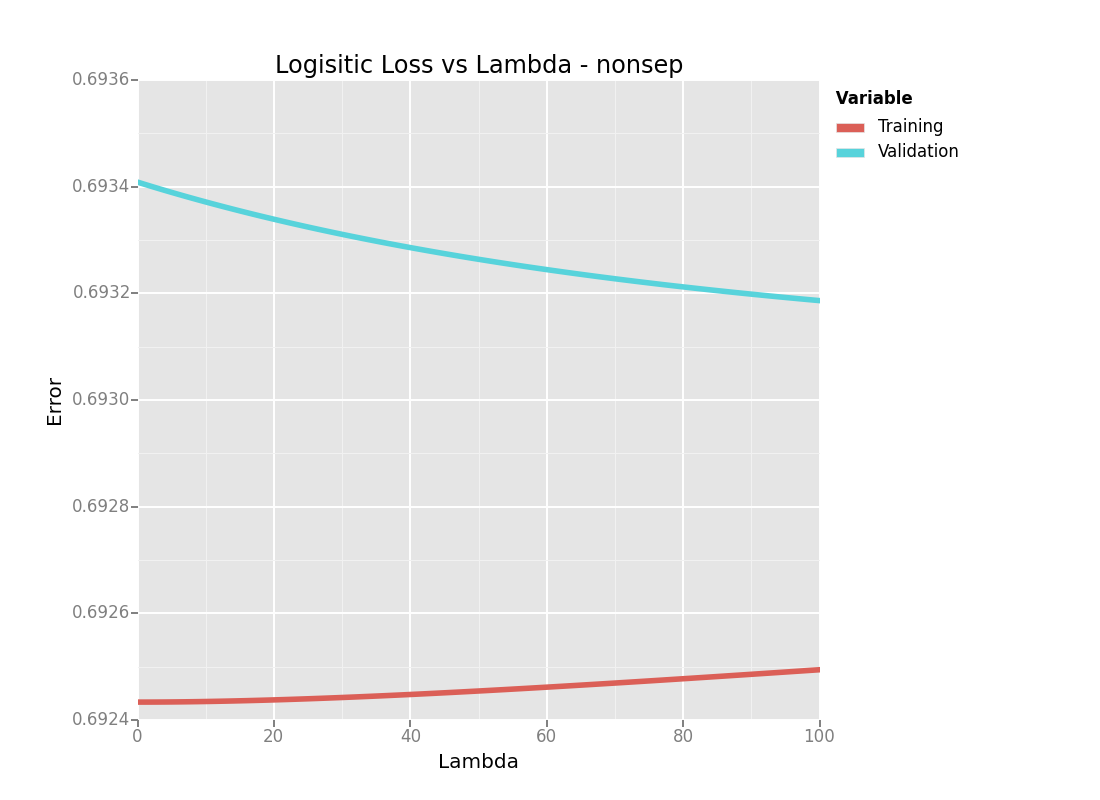
\includegraphics[width=.5\linewidth, height=.5in]{Loss_lambda_nonsep.png}
		\caption*{Logistic Loss - nonsep}
	\end{minipage}
	\caption{Classification Error (for a decision boundary of 0.5) and Loss of Logistic Regression as a function of the L2 penalty $\lambda$}
\end{figure}

We see that generally speaking, the classification error on the validation set decreases (except in the linearly separable case, where it stays at 0) as we increase our ridge penalty which is something we might expect if we think there's possible overfitting. We also see that generally speaking, loss monotonically increases with lambda, something we should expect since the ridge penalty is pushing the weights toward 0 causing logistic regression to output probabilities closer to 0.5.

\subsubsection*{Support Vector Machines}

Let's now compare the performance of SVM to that of logistic regression for classification problems. To illustrate the objective and constraints of the support vector machine, we have included below the explicit objective we would optimize over, as well as the constraints, for the dual form of a linear SVM with slack variables. The equations below correspond to the 2D problem where we have positive examples (1, 2), (2, 2) and negative examples (0, 0), (-2, 3).

\[
\min_{\alpha_1, \alpha_2, \alpha_3, \alpha_4}
\frac{1}{2}
\begin{bmatrix}
    \alpha_1 & \alpha_2 & \alpha_3 & \alpha_4 \\
\end{bmatrix}
\begin{bmatrix}
    5       & 6 & 0 & -4 \\
    6       & 8 & 0 & -2 \\
    0       & 0 & 0 & 0 \\
    -4       & -2 & 0 & 13 \\
\end{bmatrix}
\begin{bmatrix}
    \alpha_1 \\
    \alpha_2 \\
    \alpha_3 \\
    \alpha_4 \\
\end{bmatrix} 
+
\begin{bmatrix}
    -1       & -1 & -1 & -1 \\
\end{bmatrix}
\begin{bmatrix}
    \alpha_1 \\
    \alpha_2 \\
    \alpha_3 \\
    \alpha_4 \\
\end{bmatrix} 
\]

\begin{center}
s.t.
\end{center}

\[
\begin{bmatrix}
    -1 & 0 & 0 & 0 \\
    0 & -1 & 0 & 0 \\
    0 & 0 & -1 & 0 \\
    0 & 0 & 0 & -1 \\
    1 & 0 & 0 &0 \\
    0 & 1 & 0 & 0 \\
    0 & 0 & 1 & 0 \\
    0 & 0 & 0 & 1 \\
\end{bmatrix}
\begin{bmatrix}
    \alpha_1 \\
    \alpha_2 \\
    \alpha_3 \\
    \alpha_4 \\
\end{bmatrix} 
\leq
\begin{bmatrix}
0 \\
0 \\ 
0 \\ 
0 \\ 
C \\
C \\ 
C \\ 
C \\
\end{bmatrix},
\]

\[
\begin{bmatrix}
    1 & 1 & -1 & -1 \\
\end{bmatrix}
\begin{bmatrix}
    \alpha_1 \\
    \alpha_2 \\
    \alpha_3 \\
    \alpha_4 \\
\end{bmatrix} 
= 0
\]

Table 3 shows the weights generated by our soft SVM algorithm, as well as its performance on the training and validation sets, given the four datasets we've been provided for testing. The soft SVM, in this case, uses a simple linear kernel, so the decision boundaries that are generated are still straight lines in $\mathbb{R}^2$. However, the slack provided by the soft SVM allows the algorithm to classify data and create a ``margin", even when the data is not linearly separable. As expected, in general the algorithm does slightly better on the training set than the validation set. We plot our linear SVM classifier below:

\begin{figure}[ht]
	\centering
	\begin{minipage}[b]{.24\linewidth}
		\centering
		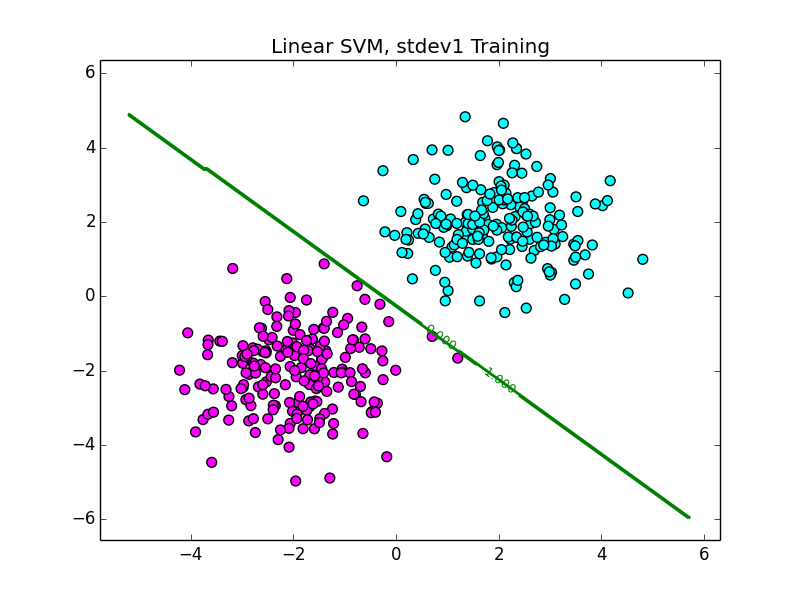
\includegraphics[width=.5\linewidth, height=.5in]{linear_svm_stdev1_train.png}
		\caption*{stdev1 (Training)}
	\end{minipage}
	\begin{minipage}[b]{.24\linewidth}
		\centering
		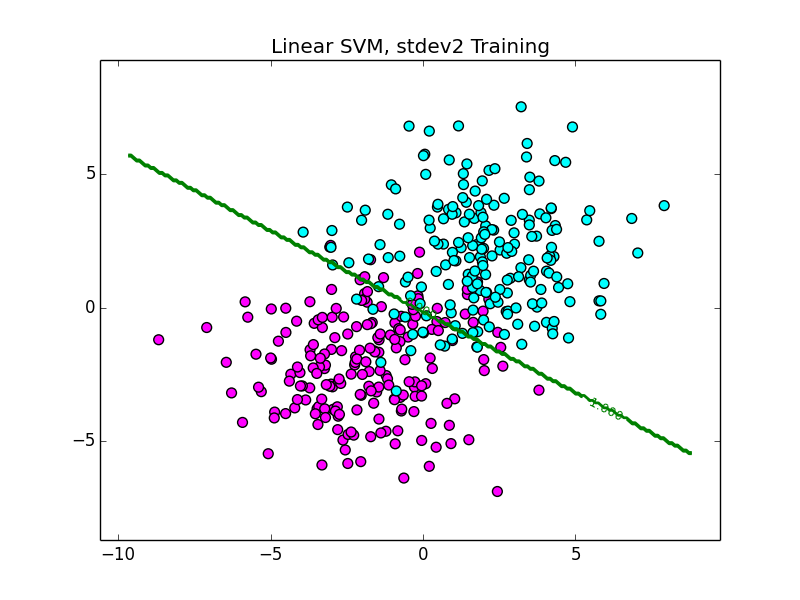
\includegraphics[width=.5\linewidth, height=.5in]{linear_svm_stdev2_train.png}
		\caption*{stdev2 (Training)}
	\end{minipage}
	\begin{minipage}[b]{.24\linewidth}
		\centering
		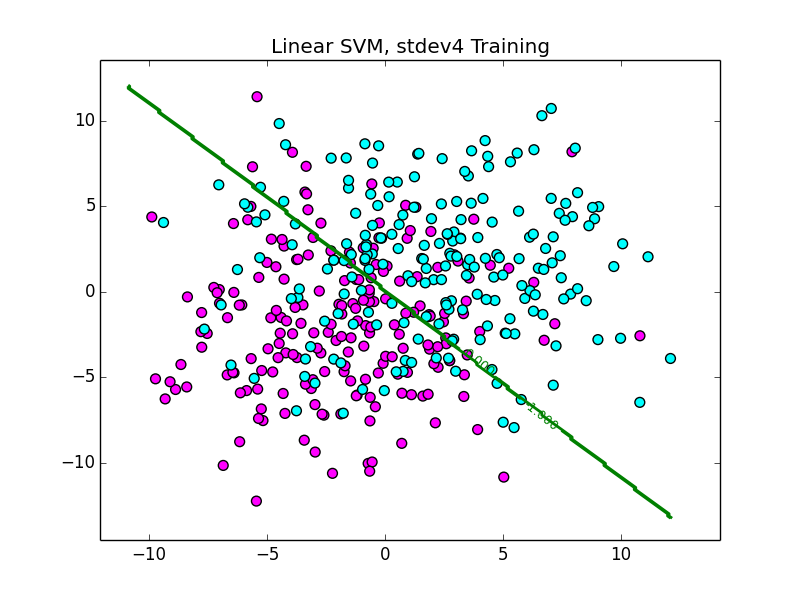
\includegraphics[width=.5\linewidth, height=.5in]{linear_svm_stdev4_train.png}
		\caption*{stdev4 (Training)}
	\end{minipage}
	\begin{minipage}[b]{.24\linewidth}
		\centering
		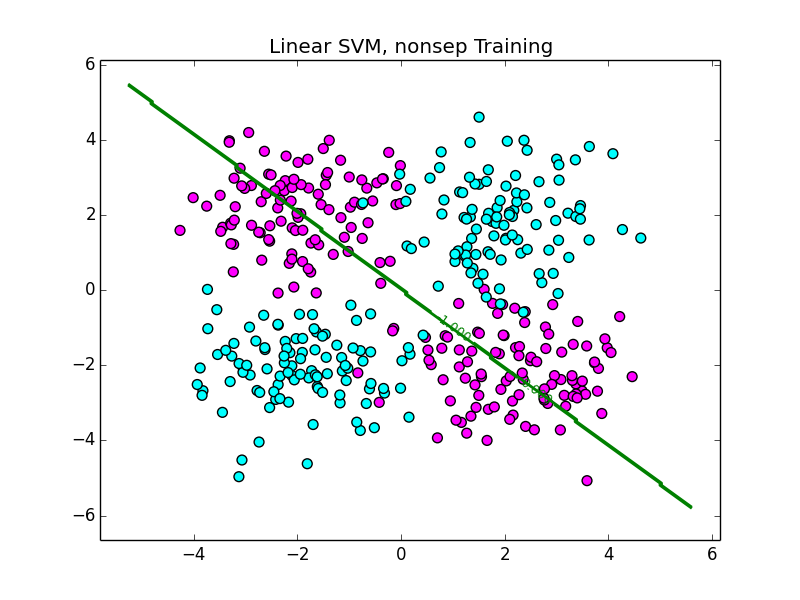
\includegraphics[width=.5\linewidth, height=.5in]{linear_svm_nonsep_train.png}
		\caption*{nonsep (Training)}
	\end{minipage}
		\begin{minipage}[b]{.24\linewidth}
		\centering
		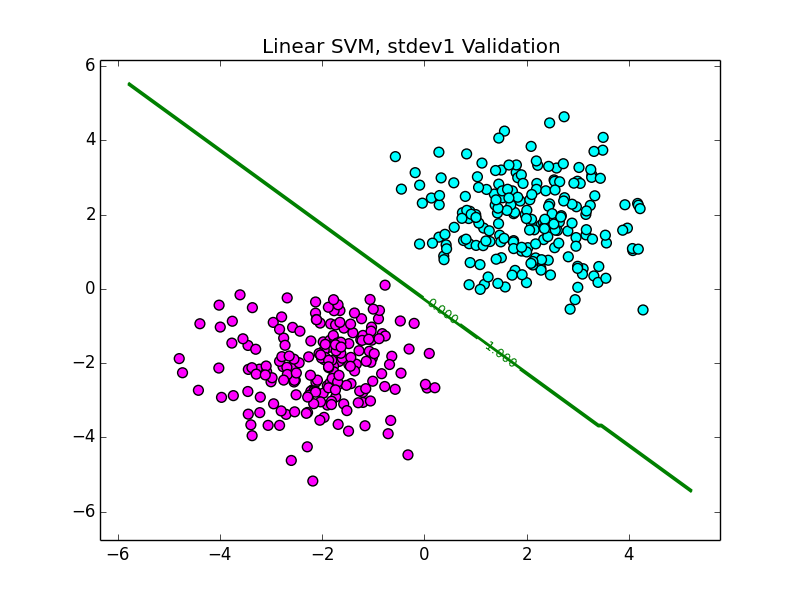
\includegraphics[width=.5\linewidth, height=.5in]{linear_svm_stdev1_validation.png}
		\caption*{stdev1 (Validation)}
	\end{minipage}
	\begin{minipage}[b]{.24\linewidth}
		\centering
		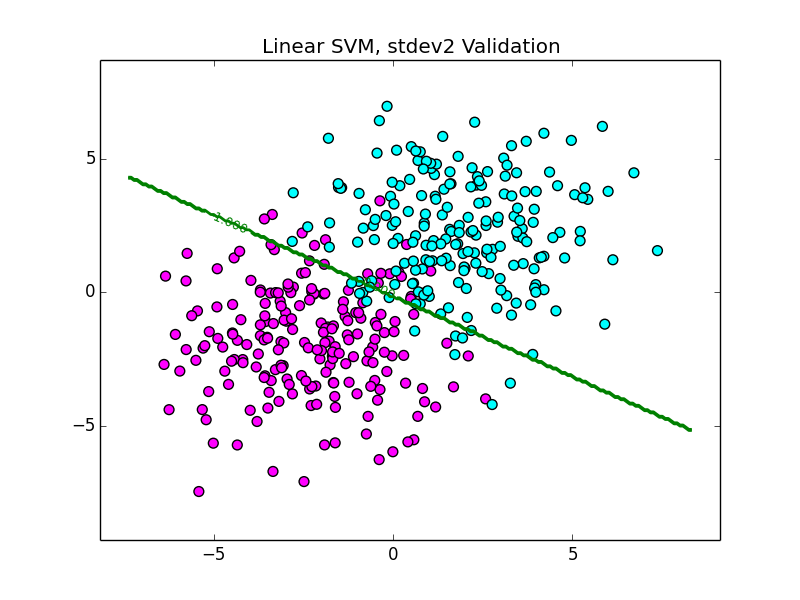
\includegraphics[width=.5\linewidth, height=.5in]{linear_svm_stdev2_validation.png}
		\caption*{stdev2 (Validation)}
	\end{minipage}
	\begin{minipage}[b]{.24\linewidth}
		\centering
		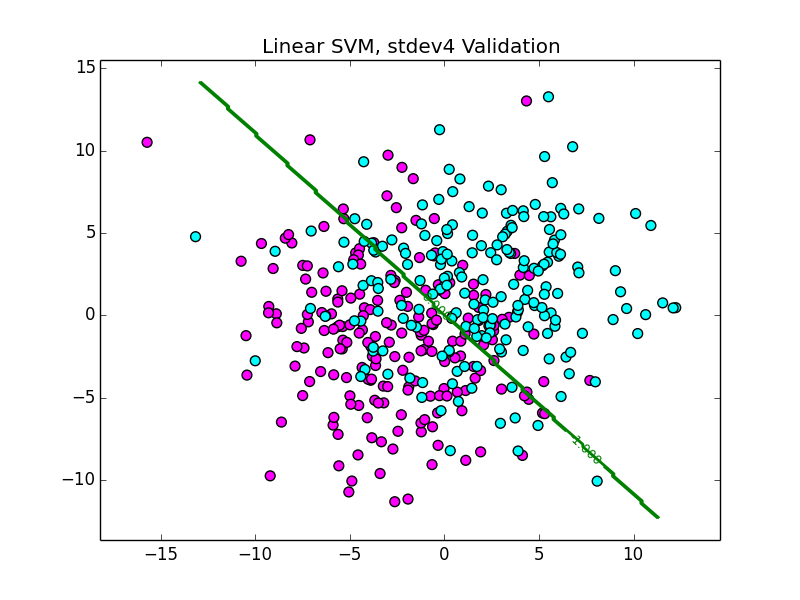
\includegraphics[width=.5\linewidth, height=.5in]{linear_svm_stdev4_validation.png}
		\caption*{stdev4 (Validation)}
	\end{minipage}
	\begin{minipage}[b]{.24\linewidth}
		\centering
		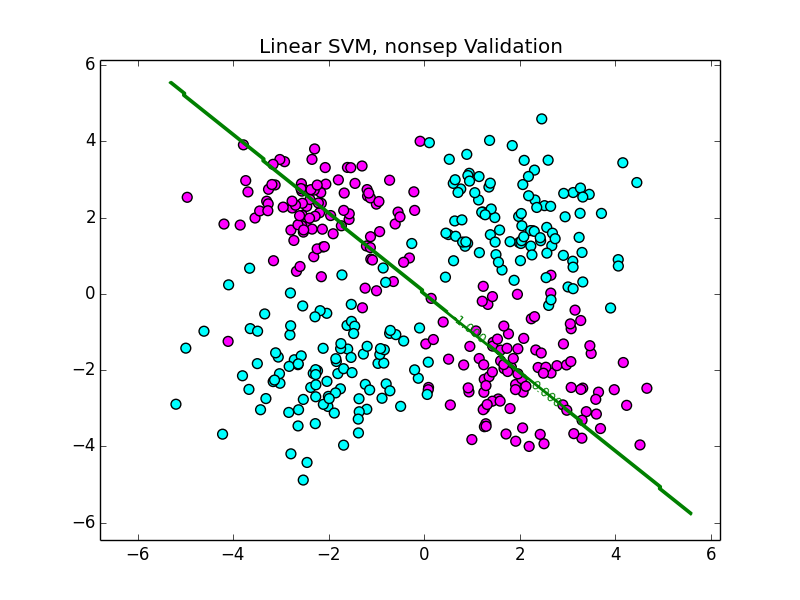
\includegraphics[width=.5\linewidth, height=.5in]{linear_svm_nonsep_validation.png}
		\caption*{nonsep (Validation)}
	\end{minipage}
	\caption{The decision boundaries generated by SVM plotted against the stdev1, stdev2, stdev4, and nonsep (training and validation) datasets}
\end{figure}

However, note that as the data becomes less and less linearly separable, our soft SVM with a linear kernel does increasingly poorly. This motivates our decision to explore the use of a Gaussian (or RBF) kernel. Table 4 includes the performance of our soft SVM algorithm on various training sets when we change kernels (for both linear and Gaussian kernels), and also when we modify the bandwidth of our Gaussian kernel (where applicable) and change our regularization parameter, $C$. 

In general, our geometric margin increases as we decrease $C$. This is to be expected - as we provide the SVM with more slack, it is able to allow more points within its margin, and can consequently expand its geometric margin. In general, the larger the geometric margin, the more support vectors - again, this is intuitive. The more slack we allow, the more data points we will observe on or inside of our margin. It is not, however, necessarily true that the geometric margin will continue to increase as we decrease $C$ (and also, geometric margin will not always decrease as we increase $C$). As C gets very large, our decision boundary will approach the hard SVM decision boundary, and will not move at all. As $C$ gets increasingly small, the additional slack will lead our decision boundary to encompass all of the data, at which point our geometric margin will stop increasing.

Choosing $C$ by maximizing the geometric margin on the training data not a mistake that a practitioner should make. This is because maximizing the geometric margin on the training data is, in a sense, overfitting on the training data. Smaller $C$ would almost always give us larger geometric margins, and the practitioner would feel compelled to choose a very small $C$. However, this choice of $C$ may lead to very poor performance on validation sets, or future data. The best method for selecting $C$ would be to perform some sort of cross-validation. In the most basic sense, we might perform a grid search with various values of C, train our soft SVM, and see which value of C provides the best performance on a held-out validation set.



\begin{table}
\centering
\captionof{table}{Classification Performance of Linear SVM}
\begin{tabular}{c c|c|c|c|c|c}
\toprule
{} & dataset & $w_0$ & $w_1$ & $w_2$ & Training Error & Validation Error \\
\midrule
  & stdev1 & 0.31 & 5.42 & 0.87 & 0.00\% & 0.00\% \\
  & stdev2 & 9.09e-2 & 9.83e1 & 9.11e1 & 9.50\% & 7.50\% \\
  & stdev4 & -2.05e-2 & 2.58e2 & 2.40e2 & 26.00\% & 23.50\% \\
  & nonsep & 2.56e-3 & 4.23e2 & 3.84e2 & 49.50\% & 51.25\% \\
\bottomrule
\end{tabular}
\end{table}

\begin{table}
\captionof{table}{Soft SVM Performance for Different Parameters and Kernels} 
\centering
\begin{tabular}{llllll}
\toprule
{} &                        Kernel &      $C$ &   $\sigma$ &    \# SV & $1/||\mathbf{w}||$ \\
\midrule
&    Gaussian &    .01 &    .1 &   400 &    .0286 \\
&    Gaussian &    .01 &    1 &   400 &    .0286 \\
&    Gaussian &    .01 &    10 &   400 &    .0286 \\
&    Gaussian &    .1 &    .1 &   400 &    .0141 \\
&    Gaussian &    .1 &    1 &   400 &    .0207 \\
&    Gaussian &    .1 &    10 &   400 &    .0141 \\
&    Gaussian &    1 &    .1 &   391 &    .0022 \\
&    Gaussian &    1 &    1 &   100 &    .0076 \\
&    Gaussian &    1 &    10 &   368 &    .0018 \\
&    Gaussian &    10 &    .1 &   390 &    .0018 \\
&    Gaussian &    10 &    1 &   71 &    .0017 \\
&    Gaussian &    10 &    10 &   209 &    .0003 \\
&    Gaussian &    100 &    .1 &   390 &    .0018 \\
&    Gaussian &    100 &    1 &   59 &    .0002 \\
&    Gaussian &    100 &    10 &   159 &    7.51e-5 \\
&    Linear &    .01 &    N/A &   399 &    .0282 \\
&    Linear &    .1 &    N/A &   393 &    .0133 \\
&    Linear &    1 &    N/A &   392 &    .0017 \\
&    Linear &    10 &    N/A &   393 &    .0002 \\
&    Linear &    100 &    N/A &   397 &    1.8e-5 \\
\midrule
\bottomrule
\end{tabular}
\end{table}


\subsubsection*{Titanic Data}
We're interested in now testing the performance of our classifiers on a real dataset. In this case, we are using the Titanic dataset, where we're assigned with the rather macabre task of predicting passenger survival given his or her features. For this problem we first scale all the features so they lie between $[0,1]$. We accomplish this by taking each observation and transforming it via:
\begin{equation*}
	x_{i,j}^* = \frac{x_{i,j}-\min(x_j)}{\max(x_j) - \min(x_j)}
\end{equation*}
This scaling of our data ensures that logistic regression behaves nicely. Otherwise, we encounter precision loss errors that end up significantly impacting our predictive accuracy. 

Using this transformed data, we train a logistic regression, a linear SVM, a polynomial SVM ($K(x,z) = (1+x\cdot z)^3$), and a gaussian SVM. For each classifier, we perform a grid search to choose the optimal hyperparameters that minimize the classification error of the validation set. We find that for logistic regression,  $\lambda = 0.38$. For linear SVM, $C=0.07$. For polynomial SVM, $C=0.03$. And for Gaussian SVM, $\sigma = 1$ and $C=0.04$.

The results generated by these settings, as well as the weights generated by these settings, are found in Tables 5 and 6. Note that we omit our bias term, $w_0$, although it is included in the model, since it does not have any immediate physical interpretation (other than perhaps the baseline rate at which people survived the sinking of the Titanic). 

\begin{table}[ht]
\centering
\captionof{table}{Titanic Data Classification Performance}
\begin{tabular}{lrrrr}
\toprule
{} & Logit & L-SVM & P-SVM & G-SVM \\
\midrule
Penalty & $\lambda = 0.38$ & $C = 0.07$ & $C = 0.03$ & $C = 0.04$\\
\midrule
Training Error    &  0.165 &  0.225 & 0.140 &  0.195 \\
Validation Error  &  0.208 &  0.208 & 0.222 &  0.210 \\
Test Error        &  0.249 &  0.233 & 0.265 &  0.243 \\
Geometric Margin  & {}     &  0.0055& 0.0112& 0.0063 \\
\bottomrule
\end{tabular}
\end{table}

As can be seen in Table 5, logistic regression outperforms polynomial SVM, with a test error rate of 24.9\% (as opposed to 26.5\% the SVM). Gaussian SVM performs outperforms the logistic regression, with a test error rate of 24.3\%, and the linear SVM performs the best, with a test error rate of 23.3\%. This is an interesting, and somewhat surprising result, as we might expect Gaussian SVM to perform as well (if not better) than linear SVM.

To better understand the differences in our models, one can look at Table 6, which reports the calculated weights for each of our trained models. We also depict this visually in Figure 5. Note that in Figure 5, each model's array of weights is normalized so that its maximum weight (in this case, always gender) is equal to 1. One can see that the linear SVM places almost all of its weight on gender, with a small amount on \# of parents/children. Logistic regression also places the most weight on gender, but also puts significant weight on (in order of decreasing magnitude) 3rd class passengers, age, \# of parents and children, 1st class passengers, and 2nd class passengers. The polynomial SVM puts most weight on passenger class and passenger embarkation locations. And the Gaussian SVM, after age, places the most weight on 3rd class passengers, 2nd class passengers, and passengers who embarked in Cherbourg.

\begin{table}[ht]
\centering
\captionof{table}{Optimal Weight Table}
\begin{tabular}{lrrrr}
\toprule
{} & Logit & L-SVM & P-SVM & G-SVM \\
\midrule
Penalty & $\lambda = 0.38$ & $C = 0.07$ & $C = 0.03$ & $C = 0.04$\\
\midrule
$w_1$  &  0.603693 &  0.031302 & -0.012892 &  0.120059 \\
$w_2$  &  0.455286 &  0.033952 & -0.010501 &  0.255103 \\
$w_3$  & -1.058978 & -0.065245 &  0.023511 & -0.375139 \\
$w_4$  &  2.475588 &  1.901134 &  0.101932 &  1.440000 \\
$w_5$  & -0.914359 & -0.078502 & -0.009049 & -0.068269 \\
$w_6$  & -0.251056 & -0.011503 &  0.000163 & -0.036648 \\
$w_7$  &  0.538155 &  0.131051 &  0.010683 &  0.104903 \\
$w_8$  &  0.330644 &  0.057787 & -0.001549 &  0.117515 \\
$w_9$  & -0.233114 & -0.038255 & -0.009864 & -0.159978 \\
$w_{10}$ &  0.291611 &  0.029324 &  0.024844 &  0.240000 \\
$w_{11}$ & -0.058496 &  0.008941 & -0.014863 & -0.080000 \\
\bottomrule
\end{tabular}	
\end{table}

\begin{figure}[ht]
	\centering
	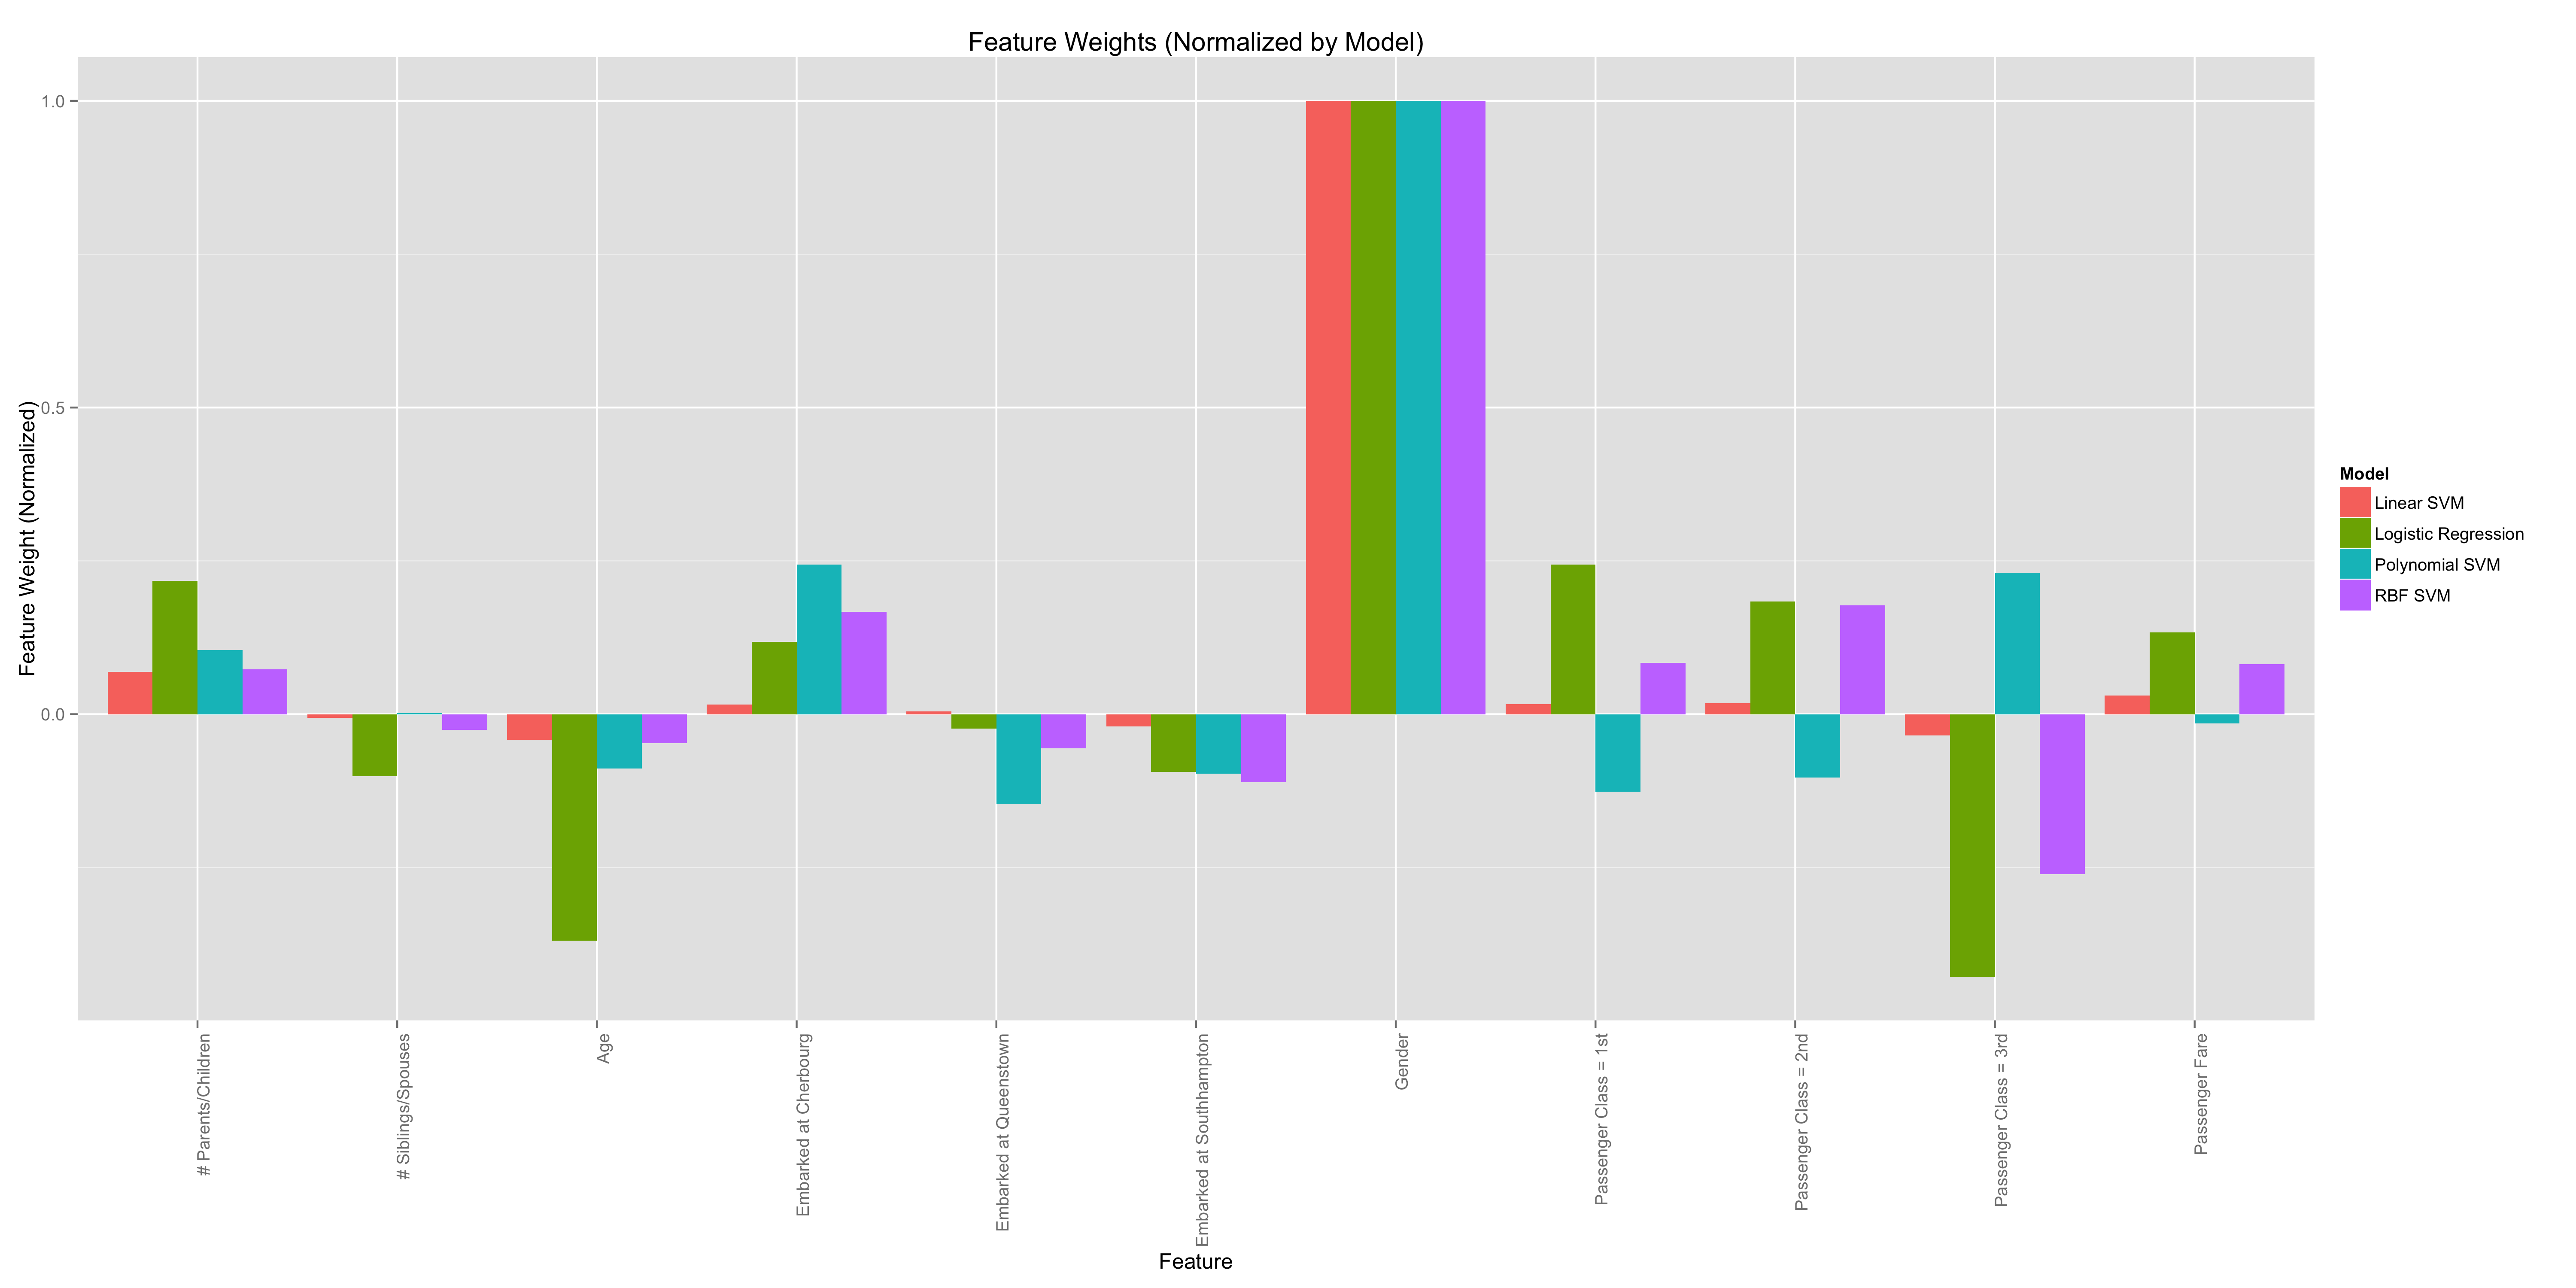
\includegraphics[height=3in]{titanic_weight_comparison.png}
	\caption*{Figure 5: Comparison of Feature Weights Across Models (Normalized per Model)}
\end{figure}

\end{document}